\documentclass{standalone}
\usepackage{tikz}
\usetikzlibrary{patterns, positioning}


\begin{document}
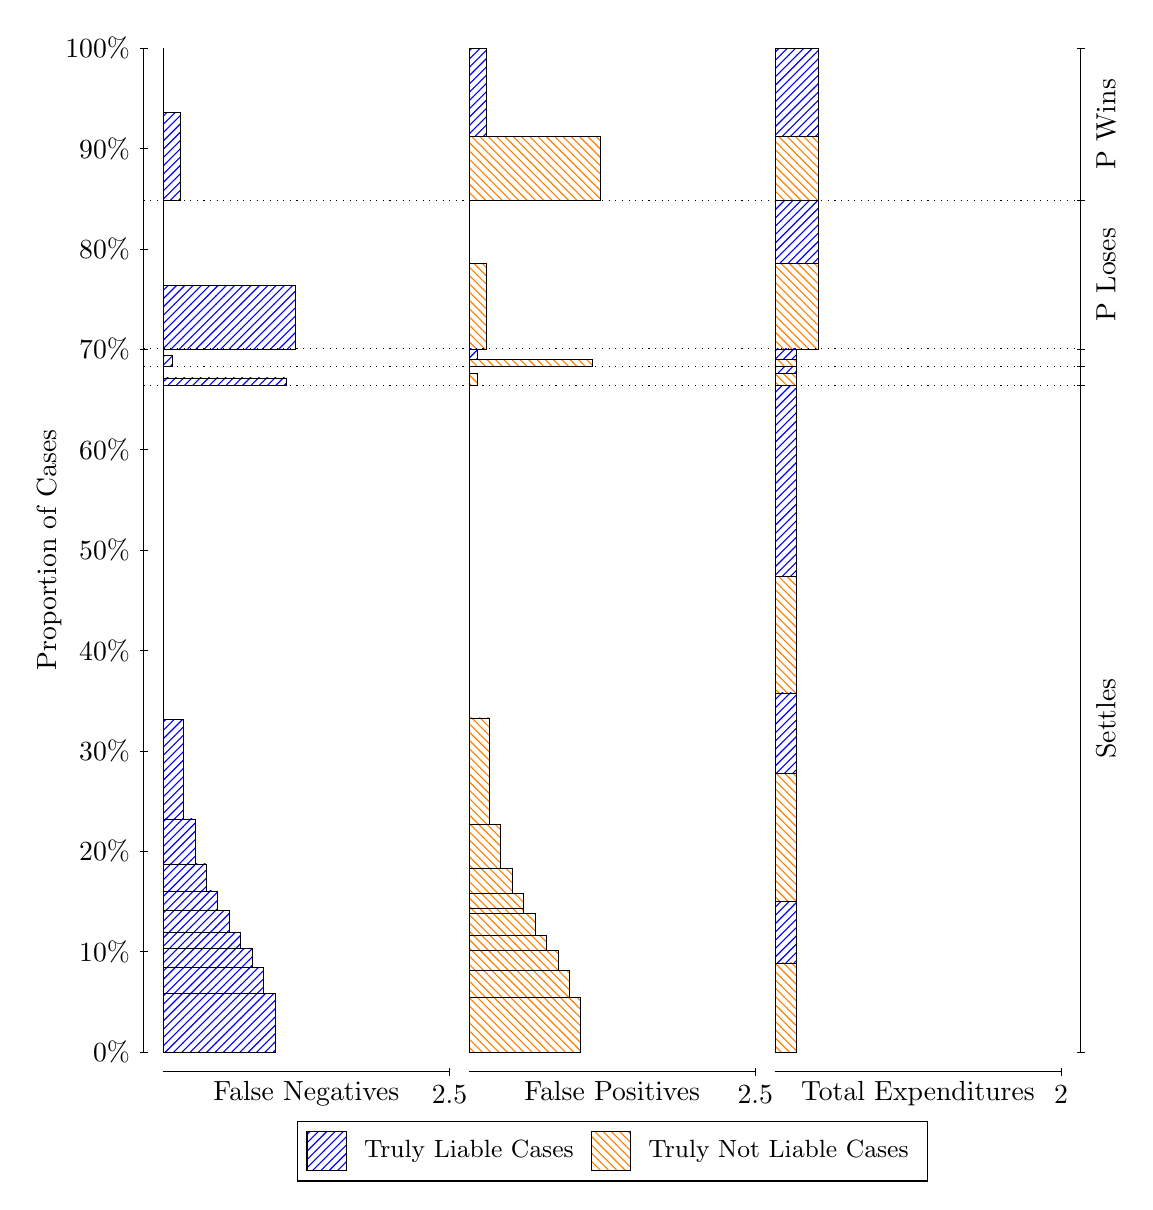
\begin{tikzpicture}
\draw[black, very thin] (1.5,1.75) -- (1.5,14.5);
\node[rotate=90, text=black, anchor=center] at (0.3, 8.125) {Proportion of Cases};
\draw[black, very thin] (1.45,1.75) -- (1.55,1.75);
\node[text=black, anchor=east] at (1.45, 1.75) {0\%};
\draw[black, very thin] (1.45,3.025) -- (1.55,3.025);
\node[text=black, anchor=east] at (1.45, 3.025) {10\%};
\draw[black, very thin] (1.45,4.3) -- (1.55,4.3);
\node[text=black, anchor=east] at (1.45, 4.3) {20\%};
\draw[black, very thin] (1.45,5.575) -- (1.55,5.575);
\node[text=black, anchor=east] at (1.45, 5.575) {30\%};
\draw[black, very thin] (1.45,6.85) -- (1.55,6.85);
\node[text=black, anchor=east] at (1.45, 6.85) {40\%};
\draw[black, very thin] (1.45,8.125) -- (1.55,8.125);
\node[text=black, anchor=east] at (1.45, 8.125) {50\%};
\draw[black, very thin] (1.45,9.4) -- (1.55,9.4);
\node[text=black, anchor=east] at (1.45, 9.4) {60\%};
\draw[black, very thin] (1.45,10.675) -- (1.55,10.675);
\node[text=black, anchor=east] at (1.45, 10.675) {70\%};
\draw[black, very thin] (1.45,11.95) -- (1.55,11.95);
\node[text=black, anchor=east] at (1.45, 11.95) {80\%};
\draw[black, very thin] (1.45,13.225) -- (1.55,13.225);
\node[text=black, anchor=east] at (1.45, 13.225) {90\%};
\draw[black, very thin] (1.45,14.5) -- (1.55,14.5);
\node[text=black, anchor=east] at (1.45, 14.5) {100\%};

\draw[black, very thin] (13.4,1.75) -- (13.4,14.5);
\draw[black, very thin] (13.35,1.75) -- (13.45,1.75);
\node[anchor=west] at (13.35, 1.75) {};
\draw[black, very thin] (13.35,10.218) -- (13.45,10.218);
\node[anchor=west] at (13.35, 10.218) {};
\draw[black, very thin] (13.35,10.459) -- (13.45,10.459);
\node[anchor=west] at (13.35, 10.459) {};
\draw[black, very thin] (13.35,10.68) -- (13.45,10.68);
\node[anchor=west] at (13.35, 10.68) {};
\draw[black, very thin] (13.35,12.564) -- (13.45,12.564);
\node[anchor=west] at (13.35, 12.564) {};
\draw[black, very thin] (13.35,14.5) -- (13.45,14.5);
\node[anchor=west] at (13.35, 14.5) {};

\draw[black, very thin, pattern color=blue, pattern=north east lines] (1.75,1.75) rectangle (3.167,2.4894);
\draw[black, very thin, pattern color=blue, pattern=north east lines] (1.75,2.4894) rectangle (3.0217,2.8272);
\draw[black, very thin, pattern color=blue, pattern=north east lines] (1.75,2.8272) rectangle (2.8763,3.0695);
\draw[black, very thin, pattern color=blue, pattern=north east lines] (1.75,3.0695) rectangle (2.731,3.2704);
\draw[black, very thin, pattern color=blue, pattern=north east lines] (1.75,3.2704) rectangle (2.5857,3.551);
\draw[black, very thin, pattern color=blue, pattern=north east lines] (1.75,3.551) rectangle (2.4403,3.7955);
\draw[black, very thin, pattern color=blue, pattern=north east lines] (1.75,3.7955) rectangle (2.295,4.1377);
\draw[black, very thin, pattern color=blue, pattern=north east lines] (1.75,4.1377) rectangle (2.1497,4.7113);
\draw[black, very thin, pattern color=blue, pattern=north east lines] (1.75,4.7113) rectangle (2.0043,5.9763);
\draw[black, very thin, pattern color=orange, pattern=north west lines] (1.75,5.9763) rectangle (1.75,10.218);
\draw[black, very thin, pattern color=blue, pattern=north east lines] (1.75,10.218) rectangle (3.3123,10.311);
\draw[black, very thin, pattern color=orange, pattern=north west lines] (1.75,10.311) rectangle (1.75,10.459);
\draw[black, very thin, pattern color=blue, pattern=north east lines] (1.75,10.459) rectangle (1.859,10.595);
\draw[black, very thin, pattern color=orange, pattern=north west lines] (1.75,10.595) rectangle (1.75,10.68);
\draw[black, very thin, pattern color=blue, pattern=north east lines] (1.75,10.68) rectangle (3.4213,11.481);
\draw[black, very thin, pattern color=orange, pattern=north west lines] (1.75,11.481) rectangle (1.75,12.564);
\draw[black, very thin, pattern color=blue, pattern=north east lines] (1.75,12.564) rectangle (1.968,13.683);
\draw[black, very thin, pattern color=orange, pattern=north west lines] (1.75,13.683) rectangle (1.75,14.5);
\draw[black, very thin, pattern color=orange, pattern=north west lines] (5.6333,1.75) rectangle (7.0503,2.4431);
\draw[black, very thin, pattern color=orange, pattern=north west lines] (5.6333,2.4431) rectangle (6.905,2.7866);
\draw[black, very thin, pattern color=orange, pattern=north west lines] (5.6333,2.7866) rectangle (6.7597,3.0365);
\draw[black, very thin, pattern color=orange, pattern=north west lines] (5.6333,3.0365) rectangle (6.6143,3.2333);
\draw[black, very thin, pattern color=orange, pattern=north west lines] (5.6333,3.2333) rectangle (6.469,3.5123);
\draw[black, very thin, pattern color=orange, pattern=north west lines] (5.6333,3.5123) rectangle (6.3237,3.5703);
\draw[black, very thin, pattern color=orange, pattern=north west lines] (5.6333,3.5703) rectangle (6.3237,3.7595);
\draw[black, very thin, pattern color=orange, pattern=north west lines] (5.6333,3.7595) rectangle (6.1783,4.085);
\draw[black, very thin, pattern color=orange, pattern=north west lines] (5.6333,4.085) rectangle (6.033,4.6444);
\draw[black, very thin, pattern color=orange, pattern=north west lines] (5.6333,4.6444) rectangle (5.8877,5.9919);
\draw[black, very thin, pattern color=blue, pattern=north east lines] (5.6333,5.9919) rectangle (5.6333,10.218);
\draw[black, very thin, pattern color=orange, pattern=north west lines] (5.6333,10.218) rectangle (5.7423,10.366);
\draw[black, very thin, pattern color=blue, pattern=north east lines] (5.6333,10.366) rectangle (5.6333,10.459);
\draw[black, very thin, pattern color=orange, pattern=north west lines] (5.6333,10.459) rectangle (7.1957,10.544);
\draw[black, very thin, pattern color=blue, pattern=north east lines] (5.6333,10.544) rectangle (5.7423,10.68);
\draw[black, very thin, pattern color=orange, pattern=north west lines] (5.6333,10.68) rectangle (5.8513,11.763);
\draw[black, very thin, pattern color=blue, pattern=north east lines] (5.6333,11.763) rectangle (5.6333,12.564);
\draw[black, very thin, pattern color=orange, pattern=north west lines] (5.6333,12.564) rectangle (7.3047,13.381);
\draw[black, very thin, pattern color=blue, pattern=north east lines] (5.6333,13.381) rectangle (5.8513,14.5);
\draw[black, very thin, pattern color=orange, pattern=north west lines] (9.5167,1.75) rectangle (9.7892,2.8821);
\draw[black, very thin, pattern color=blue, pattern=north east lines] (9.5167,2.8821) rectangle (9.7892,3.6631);
\draw[black, very thin, pattern color=orange, pattern=north west lines] (9.5167,3.6631) rectangle (9.7892,5.2896);
\draw[black, very thin, pattern color=blue, pattern=north east lines] (9.5167,5.2896) rectangle (9.7892,6.3096);
\draw[black, very thin, pattern color=orange, pattern=north west lines] (9.5167,6.3096) rectangle (9.7892,7.7929);
\draw[black, very thin, pattern color=blue, pattern=north east lines] (9.5167,7.7929) rectangle (9.7892,10.218);
\draw[black, very thin, pattern color=orange, pattern=north west lines] (9.5167,10.218) rectangle (9.7892,10.366);
\draw[black, very thin, pattern color=blue, pattern=north east lines] (9.5167,10.366) rectangle (9.7892,10.459);
\draw[black, very thin, pattern color=orange, pattern=north west lines] (9.5167,10.459) rectangle (9.7892,10.544);
\draw[black, very thin, pattern color=blue, pattern=north east lines] (9.5167,10.544) rectangle (9.7892,10.68);
\draw[black, very thin, pattern color=orange, pattern=north west lines] (9.5167,10.68) rectangle (10.062,11.763);
\draw[black, very thin, pattern color=blue, pattern=north east lines] (9.5167,11.763) rectangle (10.062,12.564);
\draw[black, very thin, pattern color=orange, pattern=north west lines] (9.5167,12.564) rectangle (10.062,13.381);
\draw[black, very thin, pattern color=blue, pattern=north east lines] (9.5167,13.381) rectangle (10.062,14.5);
\draw[black, dotted] (1.5,10.218) -- (13.4,10.218);
\draw[black, dotted] (1.5,10.459) -- (13.4,10.459);
\draw[black, dotted] (1.5,10.68) -- (13.4,10.68);
\draw[black, dotted] (1.5,12.564) -- (13.4,12.564);
\draw[black, very thin] (1.75,1.5) -- (5.3833,1.5);
\node[text=black, anchor=north] at (3.5667, 1.5) {False Negatives};
\draw[black, very thin] (5.3833,1.45) -- (5.3833,1.55);
\node[text=black, anchor=north] at (5.3833, 1.45) {2.5};

\draw[black, very thin] (5.6333,1.5) -- (9.2667,1.5);
\node[text=black, anchor=north] at (7.45, 1.5) {False Positives};
\draw[black, very thin] (9.2667,1.45) -- (9.2667,1.55);
\node[text=black, anchor=north] at (9.2667, 1.45) {2.5};

\draw[black, very thin] (9.5167,1.5) -- (13.15,1.5);
\node[text=black, anchor=north] at (11.333, 1.5) {Total Expenditures};
\draw[black, very thin] (13.15,1.45) -- (13.15,1.55);
\node[text=black, anchor=north] at (13.15, 1.45) {2};

\node[text=black, centered, rotate=90] at (13.72, 5.9841) {Settles};


\node[text=black, centered, rotate=90] at (13.72, 11.622) {P Loses};
\node[text=black, centered, rotate=90] at (13.72, 13.532) {P Wins};

\draw (7.449999999999999,1.5) node[draw=none] (baseCoordinate) {};
\begin{scope}[align=center]
        \matrix[scale=0.5, draw=black, below=0.5cm of baseCoordinate, nodes={draw}, column sep=0.1cm]{
            \node[rectangle, draw, minimum width=0.5cm, minimum height=0.5cm, pattern color=blue, pattern=north east lines] {}; &
            \node[draw=none, font=\small, text=black] (B) {Truly Liable Cases}; &
            \node[rectangle, draw, minimum width=0.5cm, minimum height=0.5cm, pattern color=orange, pattern=north west lines] {}; &
            \node[draw=none, font=\small, text=black] (B) {Truly Not Liable Cases}; \\
            };
\end{scope}

\end{tikzpicture}
\end{document}